%%%%%%%%%%%%%%%%%%%%%%%%%%%%%%%%%%%%%%%%%
% Thin Sectioned Essay
% LaTeX Template
% Version 1.0 (3/8/13)
%
% This template has been downloaded from:
% http://www.LaTeXTemplates.com
%
% Original Author:
% Nicolas Diaz (nsdiaz@uc.cl) with extensive modifications by:
% Vel (vel@latextemplates.com)
%
% License:
% CC BY-NC-SA 3.0 (http://creativecommons.org/licenses/by-nc-sa/3.0/)
%
%%%%%%%%%%%%%%%%%%%%%%%%%%%%%%%%%%%%%%%%%

%----------------------------------------------------------------------------------------
%	PACKAGES AND OTHER DOCUMENT CONFIGURATIONS
%----------------------------------------------------------------------------------------
\documentclass[12pt]{article} % Font size (can be 10pt, 11pt or 12pt) and paper size (remove a4paper for US letter paper)
\usepackage[protrusion=true,expansion=true]{microtype} % Better typography
\usepackage[left=1in,right=1in,top=1in,bottom=1in]{geometry}
\usepackage{graphicx} % Required for including pictures
\usepackage{wrapfig} % Allows in-line images
%\usepackage{mathpazo} % Use the Palatino font
\usepackage[T1]{fontenc} % Required for accented characters
%\linespread{1.05} % Change line spacing here, Palatino benefits from a slight increase by default
%\usepackage{array}
%\usepackage{booktabs}
%\usepackage{latexsym}
\usepackage{fancyhdr}
\usepackage{lastpage}
\usepackage[pdftex]{hyperref}
\usepackage{tipa}
\usepackage{url}
\usepackage{verbatim}
\hypersetup{
  colorlinks = true,
  urlcolor = black,
  citecolor=black,%
  filecolor=black,%
  linkcolor=black,%
  urlcolor=black     % can put red here to visualize the links
}
%\usepackage{biblatex}

\usepackage{outlines}
\usepackage{enumitem}
\usepackage{mathtools}
\usepackage{vector}
\usepackage{fixltx2e}

\usepackage{pdfpages}

\usepackage{xfrac}

\usepackage[labelfont=bf]{caption}

%\usepackage[latin1]{inputenc}
\usepackage{tikz}
\usetikzlibrary{shapes,arrows}

\newcounter{cenum}
\newcounter{cenumsaved}
\setcounter{cenumsaved}{0}
\newcommand{\labelcenum}{\arabic{cenum}.}
\newenvironment{cenumerate}%
{\begin{list}{\labelcenum}{\usecounter{cenum}}%
\setcounter{cenum}{\value{cenumsaved}}}%
{\setcounter{cenumsaved}{\value{cenum}}%
\end{list}}

\renewcommand{\outlineii}{cenumerate}

%\setenumerate[1]{label=\Roman*.}
%\setenumerate[2]{label=\Alph*.}
%\setenumerate[3]{label=\roman*.}
%\setenumerate[4]{label=\alph*.}

\makeatletter
%\renewcommand\@biblabel[1]{\textbf{#1.}} % Change the square brackets for each bibliography item from '[1]' to '1.'
\renewcommand{\@listI}{\itemsep=0pt} % Reduce the space between items in the itemize and enumerate environments and the bibliography

\renewcommand{\maketitle}{ % Customize the title - do not edit title and author name here, see the TITLE block below
\begin{center} % Right align
{\noindent\@title} % Increase the font size of the title

\vspace{10pt} % Some vertical space between the title and author name

{\noindent\@author}\\\@date

\vspace{10pt} % Some vertical space between the author block and abstract
\end{center}
}


\let\oldhat\hat
\renewcommand{\vec}[1]{\mathbf{#1}}
\renewcommand{\hat}[1]{\oldhat{\mathbf{#1}}}


\providecommand{\e}[1]{\ensuremath{\times 10^{#1}}}

%----------------------------------------------------------------------------------------
%	TITLE
%----------------------------------------------------------------------------------------
%\title{\LARGE{\textbf{Software Engineering Best Practices\\in Biomedical Informatics}\\[.5em]
%}}
%
%\author{\large{Nicholas J. Matiasz}\vspace{.4em}}
%
%\date{\large{2013-10-31}} % Date
%----------------------------------------------------------------------------------------

%----------------------------------------------------------------------------------------
%	HEADER/FOOTER
%----------------------------------------------------------------------------------------
\lhead{}
\chead{}
\rhead{}
\lfoot{BE 224A \textpipe\ X-ray Simulation}
\cfoot{\thepage\ of\ \pageref{LastPage}}
\rfoot{Nicholas J. Matiasz}
\renewcommand{\headrulewidth}{0.4pt}
\renewcommand{\footrulewidth}{0.4pt}
\pagestyle{fancyplain}



%----------------------------------------------------------------------------------------
%	ESSAY BODY
%----------------------------------------------------------------------------------------
\begin{document}

\begin{titlepage}

\newcommand{\HRule}{\rule{\linewidth}{0.5mm}} % Defines a new command for the horizontal lines, change thickness here

\center % Center everything on the page
 
%----------------------------------------------------------------------------------------
%	HEADING SECTIONS
%----------------------------------------------------------------------------------------

\textsc{\Large University of California, Los Angeles}\\[1.5cm] % Name of your university/college
\textsc{\large Medical Imaging Informatics Group}\\[0.5cm] % Major heading such as course name
\textsc{\large BE 224A X-ray Simulation}\\[0.5cm] % Minor heading such as course title

%----------------------------------------------------------------------------------------
%	TITLE SECTION
%----------------------------------------------------------------------------------------
\vspace{20pt}
\HRule \\[0.5cm]
\LARGE{\textbf{Monte Carlo Simulation of}}\\[.3cm]
\LARGE{\textbf{X-ray Interaction with Water Phantom}}\\
\HRule \\[1.5cm]
 
%----------------------------------------------------------------------------------------
%	AUTHOR SECTION
%----------------------------------------------------------------------------------------

\begin{minipage}{0.4\textwidth}
\begin{flushleft} \large
\emph{Author:}\\
Nicholas J.\ Matiasz % Your name
\end{flushleft}
\end{minipage}
~
\begin{minipage}{0.4\textwidth}
\begin{flushright} \large
\emph{Instructor:} \\
Prof.\ Ricky Taira % Supervisor's Name
\end{flushright}
\end{minipage}\\[4cm]

% If you don't want a supervisor, uncomment the two lines below and remove the section above
%\Large \emph{Author:}\\
%John \textsc{Smith}\\[3cm] % Your name

%----------------------------------------------------------------------------------------
%	DATE SECTION
%----------------------------------------------------------------------------------------
\begin{minipage}{0.4\textwidth}
\begin{center} \large
\emph{Submitted:} \\
2014-02-04 % Supervisor's Name
\end{center}
\end{minipage}\\[4cm]
%{\large Submitted: 2013-10-30}\\[3cm] % Date, change the \today to a set date if you want to be precise

%----------------------------------------------------------------------------------------
%	LOGO SECTION
%----------------------------------------------------------------------------------------
%\includegraphics{Logo}\\[1cm] % Include a department/university logo - this will require the graphicx package
%----------------------------------------------------------------------------------------
\vfill % Fill the rest of the page with whitespace
\end{titlepage}


\fontsize{12}{20}%22.5, 28
\selectfont
%\thispagestyle{empty}
%\tableofcontents

\section*{Introduction}
The purpose of this exercise was to simulate a radiographic experiment in which 100,000,000 photons pass through a water phantom and strike a film plane. Descriptions of both the system and simulation follow, along with a discussion of the results.

\section*{System description}
Refer to Figure \ref{system_diagram} for a diagram of the simulated system. Let the positive $x$ direction be directed to the right in Figure \ref{system_diagram} such that, by the right-hand rule, the positive $z$-axis is directed into the page.
Each photon begins its motion in the positive $y$ direction, or ``down'' in Figure \ref{system_diagram}.
Let the point that sits along the first air/phantom boundary at the middle of the phantom be the origin of the coordinate space, where $x = 0$, and $y = 0$. The film plane is parallel to the $x$-axis, and is collinear with the line $y=d_1 + d_2$. The film plane is infinitely long, extending toward both positive and negative infinity.

\begin{figure}[h]
\centering
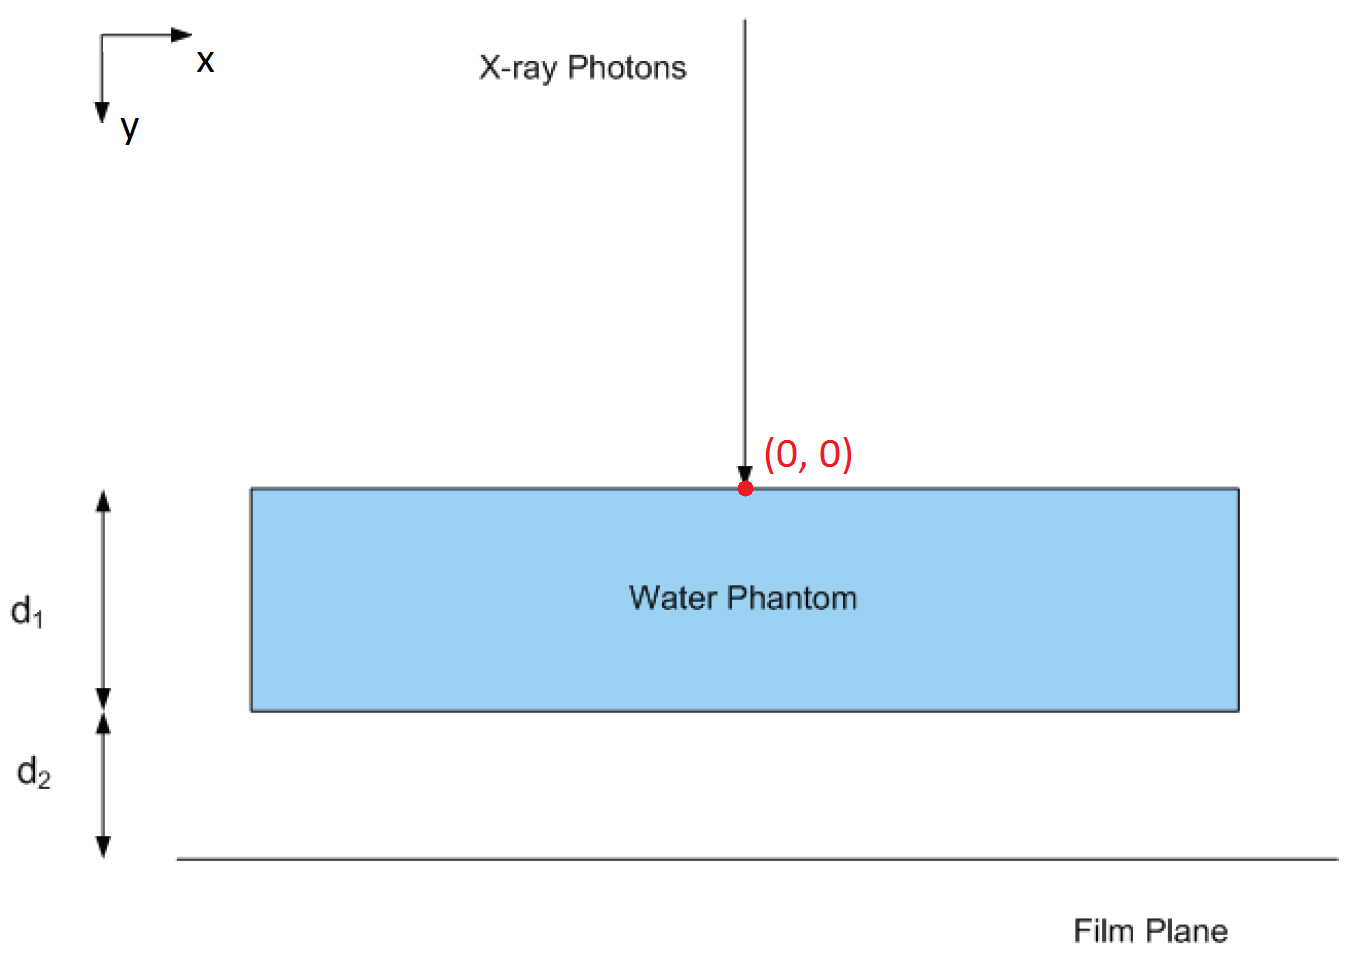
\includegraphics[scale=.5]{./images/system_diagram_2.png}
\caption{System diagram}
\label{system_diagram}
\end{figure}


\section*{Assumptions}
The following assumptions are made for this simulation:
\begin{enumerate}
\item All photon motion occurs in the $xy$\nobreakdash-plane (i.e., where $z = 0$).

\item The initial photon beam is a pencil beam, with a width that is infinitesimally small.

\item All photons are assumed to be fired in the positive y direction at $x = 0$, and continue in this straight trajectory until interacting with the phantom.

%\item The energy of the photons is uniformly distributed in the diagnostic range, namely 20--150 keV.

\item Rayleigh scattering is assumed not to occur, as this type of scattering usually occurs with low-energy x-rays in the 15--30 keV range \cite[p.~37]{bushberg2002}, which overlaps only slightly with the range of energies used in the simulation (20--150 keV).

\item Pair production is assumed not to occur, as this phenomena occurs only when an incident photon's energy exceeds 1.02~MeV \cite[p.~155]{johns1983}.

\item The x-ray photons do not interact with each other. It is therefore sufficient to simulate each photon's journey individually, with respect to no other photons. A record of each photon's behavior can be recorded to allow for aggregated statistics (e.g., percentage of photoelectric interactions).

\end{enumerate}

\section*{Considerations for simulation}
In order to simulate the interaction of x-radiation with a water phantom, the material properties of water must be considered. Table \ref{water_values} presents the values of various constants \cite[p.~142]{johns1983} that are relevant to the simulation of the water phantom depicted in Figure \ref{system_diagram}. 

%\begin{center}
\begin{table}[h]
\caption{Characteristics of water phantom}
\centering
\begin{tabular}{ c c c }
\hline\hline
  \textbf{Quantity} & \textbf{Value} & \textbf{Units} \\
  \hline
  $\rho$, density & 1000 & kg/m\textsuperscript{3} \\
  $Z_{eff}$, effective atomic number & 7.51 & \\
  N\textsubscript{e}, electrons per gram & 3.34\e{23} & g\textsuperscript{-1}\\
\end{tabular}
\label{water_values}
\end{table}
%\end{center}

Each photon is represented by a vector, where each component represents a parameter that models the photon's state.
Given that only one photon is simulated at a time, only one vector is required for all photons.
Let $n$ equal the number of parameters that are used to model the state of each photon. 
We can then define a vector $\bvec{p}$, shown in Equation \ref{vector}, to model the state of each photon.
\begin{equation}
\bvec{p} = \left[\icvec{p}\right]
\label{vector}
\end{equation}
For this simulation, $n=4$. The four parameters to be tracked for each photon are $x$, the $x$\nobreakdash-coordinate position of the photon [m], $y$, the $y$\nobreakdash-coordinate position of the photon [m], $\nu$, the frequency of the photon [s\textsuperscript{-1}], and $\alpha$, the angle in the $xy$\nobreakdash-plane along which the photon is moving [rad]. To enable the simulation, other quantities will be determined (by either sampling a distribution randomly or calculating them directly), but the above four quantities are assumed to model each photon sufficiently.

To simulate the photons' journey through space, the vector is subjected to
a sequence of calculations, each of which characterizes the particular
region(s) in space and/or nuclear event(s) it is meant to simulate. Each calculation results in one or more adjustments (or lack thereof) to the components of the vector. During and after each photon's movement through space, specific components of $\bvec{p}$ can be recorded and later aggregated for analysis.

\section*{Monte Carlo Simulation}
The flowchart in Figure \ref{monte_carlo} visualizes a Monte Carlo simulation, as explained in \cite[p.~635--7]{barrett1981}, to model the experiment described above. Below is a description of each step in the flowchart. 

\begin{itemize}
\item Determine photon's initial energy
\end{itemize}

When a new photon is created for the simulation, three of its four parameters are already determined. Both $x$ and $y$ equal zero in order to place the photon at the origin in the coordinate space. It is assumed that no modifications to the photon occur in the space prior to encountering the phantom, so it is sufficient to begin the simulation at the air/water boundary indicated in Figure \ref{system_diagram}. The value of $\alpha$ is set to $\pi/2$ radians such that the photon is traveling in the positive $y$ direction. If the distribution of photon energy that characterizes the source is known, this distribution can be randomly sampled to obtain each photon's energy, and thus its frequency, $\nu$. Otherwise, we can assume that the energy of the photons is uniformly distributed in the diagnostic range (20--150 keV), and sample from this uniform distribution.

\begin{itemize}
\item Determine whether interaction occurs in phantom; record location if interaction occurs
\end{itemize}

This simulation models the behavior of x-radiation on a per-photon basis. Thus, we can use models that assume a monoenergetic x-ray beam with a homogeneous absorber. To describe the probability of each photon interacting with the phantom, we use the transmittance function in Equation \ref{eq:transmittance}.
\begin{equation}
t_d = e^{-\mu_{tot} d}
\label{eq:transmittance}
\end{equation}
In Equation \ref{eq:transmittance}, $\mu_{tot}$ is the total linear attenuation coefficient, which is obtained by adding the linear attenuation coefficients that correspond to coherent, Compton, and photoelectric interactions.
\begin{equation}
\mu_{tot} = \mu_{coh} + \mu_{cmpt} + \mu_{pe}
\label{eq:mu_total}
\end{equation}
We are ignoring coherent scattering for this simulation, so we approximate $\mu_{tot}$ by excluding coherent scattering's attenuation contribution.
\begin{equation}
\mu_{tot} \approx \mu_{cmpt} + \mu_{pe}
\label{eq:mu_total_approx}
\end{equation}
We can calculate the value of $\mu_{cmpt}$ using Equation \ref{eq:mu_cmpt}, where $_{e}\sigma$ is the total Compton Klein-Nishina cross-section per electron, $\rho$ is the density of the absorbing material (see Table \ref{water_values}), and $N_{e}$ is the number of electrons per gram of the absorbing material (see Table \ref{water_values}).
\begin{equation}
\mu_{cmpt} = _{e}\sigma\rho N_{e}
\label{eq:mu_cmpt}
\end{equation}
If we let $\beta = \sfrac{h\nu}{m_{0}c^{2}}$, where $m_{0}$ is the mass of the recoil electron, we can calculate $_{e}\sigma$, the total Compton Klein-Nishina cross-section per electron, using Equation \ref{eq:total_compton_kn}.
\begin{equation}
_{e}\sigma = 2\pi r_{0}^{2}\left[\frac{1+\beta}{\beta^{2}}\left(\frac{2(1+\beta)}{1+2\beta} - \frac{ln(1+2\beta}{\beta}\right) + \frac{ln(1+2\beta}{2\beta} - \frac{1+3\beta}{\left(1+2\beta\right)^{2}}
\label{eq:total_compton_kn}\right]
\end{equation}
We can approximate the value of $\mu_{pe}$ using Equation \ref{eq:mu_pe}, where $k$ is an experimentally determined constant, $Z$ is the atomic number of the absorbing material (for which we can substitute $Z_{eff}$ from Table \ref{water_values}), $h$ is Planck's constant, $N_{a}$ is Avogadro's number, and $A$ is the mass number of the absorbing material.
\begin{equation}
\mu_{pe} \approx k\left(\frac{Z}{h\nu}\right)^3\rho N_{e}
\label{eq:mu_pe}
\end{equation}
Equations \ref{eq:mu_total} through \ref{eq:mu_pe} allow us to define Equation \ref{eq:transmittance} fully. We can now define the probability of a photon undergoing either a Compton or photoelectric interaction in the phantom; see Equation \ref{eq:probability_interaction}. Randomly sampling from this probability distribution will allow the simulation to determine whether each photon undergoes either a Compton or photoelectric interaction in the phantom.
\begin{equation}
\text{Pr}(\text{interaction}) = 1 - t_{d}
\label{eq:probability_interaction}
\end{equation}
\begin{itemize}
\item Calculate whether photon is on trajectory to strike film plane
\end{itemize}

If a primary photon does not interact with the phantom, or if a photon that has previously interacted with the phantom escapes the phantom, we need to determine whether the photon is on a trajectory that will allow it to strike the film plane. Given our assumption that the film plane extends infinitely in the positive and negative $x$ directions, it is sufficient to check whether the photon's value of $\alpha$ has a positive $y$ component. If it does, we can be sure that the photon will eventually strike the film plane.

\begin{itemize}
\item Calculate location at which photon strikes film plane. Record photon's energy and location on film plane
\end{itemize}

A photon that is traveling in the positive $y$ direction and that has escaped the phantom will eventually strike the film plane. It is straightforward to triangulate the photon's eventual destination on the film plane using its current position, $(x, y)$, the direction it's traveling, given by $\alpha$, and the film plane's location, which is collinear with $y = d_1 + d_2$.

\begin{itemize}
\item Discard photon's state
\end{itemize}

Photons that have escaped the phantom but that are on a trajectory in the negative $y$ direction will neither interact with the phantom nor deliver any dose; therefore, for the purposes of the simulation, such photons are irrelevant and can be discarded.

\begin{itemize}
\item Determine whether Compton or photoelectric interaction occurs
\end{itemize}
Building upon Equation \ref{eq:probability_interaction}, we can define the probabilities of a Compton interaction and of a photoelectric interaction, given in Equations \ref{eq:probability_compton} and \ref{eq:probability_photoelectric}, respectively.
\begin{equation}
\text{Pr}(\text{Compton interaction}) = \frac{\mu_{cmpt}}{\mu_{tot}}\left(1 - t_{d}\right)
\label{eq:probability_compton}
\end{equation}
\begin{equation}
\text{Pr}(\text{photoelectric interaction}) = \frac{\mu_{pe}}{\mu_{tot}}\left(1 - t_{d}\right)
\label{eq:probability_photoelectric}
\end{equation}
\begin{figure}
\centering
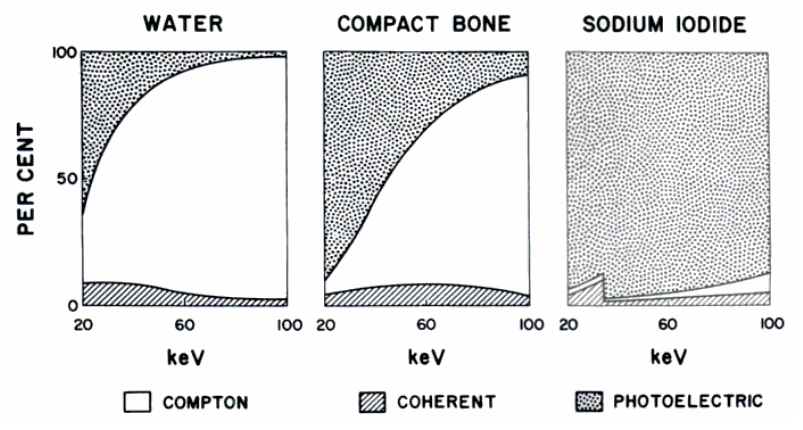
\includegraphics[scale=.75]{./images/water_interactions.png}
\caption{Occurrence of Compton, coherent, and photoelectric interactions in three different media, copied from \cite[p.~69]{curry1990})}
\label{fig:water_interactions}
\end{figure}

For a more heuristic-based approach, consider the following. The probability that a photon will undergo either a Compton or photoelectric interaction depends on multiple factors, including the photon's energy, as well as the medium in which it is traveling. Figure \ref{fig:water_interactions}, copied from \cite[p.~69]{curry1990}, displays the relative amount of Compton, coherent, and photoelectric interactions that occur in water, the material of our phantom. This empirical data can be used to model the probability of specific type of interaction occurring as a function of the photon's energy. Note that it is reasonable to replace the area of the plot corresponding to coherent interactions with additional Compton area, because, in the diagnostic energy range (20--150 kEV), coherent scattering occurs with very low probability. We can therefore approximate the curve for water in Figure \ref{fig:water_interactions} by Equation \ref{eq:probability_interaction_heuristic}.
\begin{equation}
\begin{array}{rl}y(E) = 100(1-e^{\sfrac{-E}{40}}), & 20 \le E \le 150\end{array}
\label{eq:probability_interaction_heuristic}
\end{equation}
For a given photon of known energy ($E = h\nu$), we can calculate $y(E)$, which acts as a threshold value for our simulation. Using a uniform distribution, we generate a random number, $r$, in the range $[0, 100]$. We can then compare $r$ to $y(E)$; if $r < y(E)$, the simulation determines that the photon has undergone a Compton interaction; if $r > y(E)$, the simulation determines that a photoelectric interaction has occurred. Note that for a photoelectric interaction to occur, the energy of the incident photon, $h\nu$, must be greater than the binding energy, $E_{b}$, of the atomic electron.

\pagebreak[4]
\begin{itemize}
\item Determine energy of recoil electron and scattered photon
\end{itemize}

In the case of Compton interaction, we can sample the Klein-Nishina cross section to obtain values of $\theta$ and $\phi$, which represent the angles at which the scattered photon and recoil electron depart the interaction site, respectively. These angles, along with the initial photon's value of $\alpha$, can be used to determine the trajectory of the scattered photon so that its continued journey can be further simulated. Equations \ref{eq:compton_1} through \ref{eq:compton_3}, which acknowledge the conservation of momentum, can be used to calculate the energy and angles for the scattered photon and recoil electron that result from a Compton interaction. Note that subscripts of $1$ pertain to the incident photon, and subscripts of $2$ pertain to the scattered photon. Additionally, $p_{e}$ is the momentum of the recoil electron, and $T_{e}$ is the energy of the recoil electron.
\begin{equation}
\frac{h_{1}\nu_{1}}{c} = \frac{h_{2}\nu_{2}}{c}\cos\theta + p_{e}\cos\phi
\label{eq:compton_1}
\end{equation}
\begin{equation}
0 = \frac{h_{2}\nu_{2}}{c}\sin\theta - p_{e}\cos\phi
\label{eq:compton_2}
\end{equation}
\begin{equation}
h_{1}\nu_{1} = h_{2}\nu_{2} + T_{e}
\label{eq:compton_3}
\end{equation}
\begin{itemize}
\item Record recoil electron's contribution to absorbed dose
\end{itemize}

If we assume that all of the recoil electron's energy is absorbed by the phantom, we can use the value of $T_{e}$ from Equation \ref{eq:compton_3} to record the dose contributed by the Compton interaction's recoil electron.

\begin{itemize}
\item Determine direction of scattered photon
\end{itemize}

The value of $\theta$ in Equation \ref{eq:compton_1} and the incident photon's value of $\alpha$ can be used to calculate the direction in which the scattered photon will travel.

\begin{itemize}
\item Determine energy of photoelectron
\end{itemize}

In the case of a photoelectric interaction, the ejected photoelectron will have an energy given by Equation \ref{eq:photoelectric_energy}, where $\nu$ is the frequency of the incident photon and $\nu_{0}$ is the threshold frequency of the absorbing material.

\begin{equation}
E_{pe} \le h\left(\nu - \nu_{0}\right)
\label{eq:photoelectric_energy}
\end{equation}

\begin{itemize}
\item Record photoelectron's contribution to absorbed dose
\end{itemize}

If we assume that all of the photoelectron's energy is absorbed by the phantom, we can use the value of $E_{pe}$ from Equation \ref{eq:photoelectric_energy} to record the dose contributed by the ejected photoelectron.

\begin{figure}
\centering
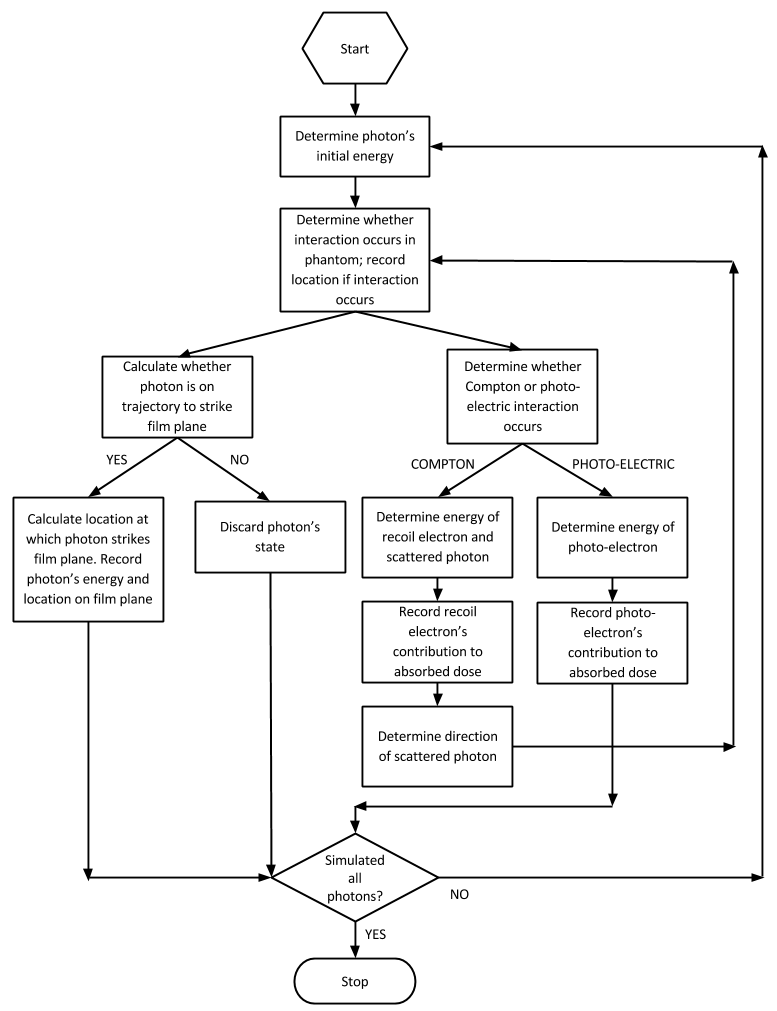
\includegraphics[scale=.575]{./images/monte_carlo.png}
\caption{Flowchart for Monte Carlo simulation}
\label{monte_carlo}
\end{figure}


\section*{Discussion}
The above simulation attempts to model the behavior of x-radiation photons as they interact with a water phantom. Despite our attempts to represent the salient aspects of this system mathematically, the model of course fails to correspond perfectly with reality. Rogers and Bielajew \cite{rogers1990} describe the various ways in which Monte Carlo code can be inadequate for modeling the behavior of photons, including uncertainty in cross-section data, unknown programming errors, modeling inaccuracies due to approximations, roundoff and truncation errors, and statistical uncertainties, specifically surrounding the use of $s^{2}$ to estimate the true variance, $\sigma^{2}$. Regarding this particular simulation, some of our largest approximation errors would result from ignoring coherent scattering, which includes approximating $\mu_{tot}$ using only $\mu_{cmpt}$ and $\mu_{pe}$. This simulation is also significantly simplified by allowing considering motion only in the $xy$\nobreakdash-plane.


%----------------------------------------------------------------------------------------
%	BIBLIOGRAPHY
%----------------------------------------------------------------------------------------
\newpage
\bibliographystyle{plain}
\bibliography{224a_xray_simulation}
%----------------------------------------------------------------------------------------

\end{document}